\documentclass[a4paper,10pt]{article} %type de document et paramètres


\usepackage{lmodern} %police de caractère
\usepackage[english,francais]{babel} %package de langues
\usepackage[utf8]{inputenc} %package fondamental
\usepackage[T1]{fontenc} %package fondamental

\usepackage[top=3cm, bottom=3cm, left=2cm, right=2cm]{geometry} %permet de paramétrer les marges par défaut
\usepackage{changepage} %permet de modifier localement une mise en page (marges,...) : utilisé pour la page de garde
%\usepackage{multicol} %permet de mettre plusieurs colonnes (\begin{multicols}{2} \end{multicols} jusqu'à 10 colonnes)
\usepackage[pdftex, pdfauthor={Pierre Gimalac}, pdftitle={Modèle}, pdfsubject={LaTeX}, pdfkeywords={LaTeX}, colorlinks=true, linkcolor=black]{hyperref} %permet de se déplacer dans le pdf depuis le sommaire en cliquant sur les titres, ainsi que de parametrer les meta données du PDF
%\usepackage{url} %permet de mettre des URL actifs \url{}
%\let\urlorig\url
%\renewcommand{\url}[1]{\begin{otherlanguage}{english}\urlorig{#1}\end{otherlanguage}}

%\usepackage{mathtools} %maths (à developper, utile par exemple pour enlever les espaces dus aux boites $\sum_{\mathclap{1\le i\le j\le n}} X_{ij}$)
%\usepackage{amssymb} %maths
%\usepackage{amsthm} %maths
%\usepackage{amsmath} %maths
%\usepackage{mathrsfs} %maths (par exemple les lettres caligraphiées)
%\usepackage{stmaryrd} %maths (par exemple les ensembles d'entiers \rrbracket \llbracket)
%\usepackage{calrsfs} %maths (par exemple les notations des ensembles)
%\usepackage{yhmath} % permet de noter les arcs de cercle avec \wideparen{AOB}
%\usepackage{xlop} %permet d'afficher des opérations mathématiques
%\usepackage[squaren,Gray]{SIunits} %permet de noter des unités proprement
%\usepackage{esdiff} %permet d'écrire la dérivée avec la notation de Leibniz \diff{v}{t}

\usepackage{graphicx} %permet d'insérer des images proprement (ajoute des parametres)
%\usepackage{wrapfig} %permet de mettre des images à coté d'un texte
%\usepackage{pdfpages} %permet d'insérer un pdf \includepdf[pages={1-2}]{truc.pdf}
\usepackage{enumitem} %permet de changer le label d'une liste \begin{itemize}[label=$\cdot$]
%\usepackage{ulem} %permet de souligner/barrer du texte
%\usepackage{soul} %permet de souligner/barrer du texte
%\usepackage{cancel} %permet de barrer du texte /cancel{text}


%\usepackage{tikz} %package trooop bien permet de dessiner tout et n'importe quoi ! \begin{tikzpicture}
%\usetikzlibrary{automata,positioning} % pour dessiner des automates
%\usepackage{circuitikz} %permet de dessiner des circuits logiques (entre autre) avec la syntaxe de tikz (\begin{circuitikz}) par exemple \node[american not port] pour le 'non'
%\usepackage{listings} %permet d'inserer du code dans le fichier (\lstset{language=Java} \begin{lstlisting} \end{lstlisting} )



\begin{document}

\begin{titlepage}
\newgeometry{margin=2.7cm}
\thispagestyle{empty}
\begin{center}
\vspace*{7cm}
\Huge \textsc{Projet informatique}\\
\vspace{1.5cm}
\Large Cahier des charges\\
\vspace{0.5cm}
\large \textit{Yushen Bai, Félix Desmaretz, Maxime Flin, Pierre Gimalac}
\end{center}
\vfill
\large \textit{Connais ton adversaire, connais-toi, et tu ne mettras pas ta victoire en danger. Connais le ciel et connais la terre, et ta victoire sera totale.}
\hfill 
\large 
\restoregeometry
\end{titlepage}

\renewcommand{\contentsname}{Sommaire}
\thispagestyle{empty}
\tableofcontents
\thispagestyle{empty}

\newpage

\section{Applications autour du jeu}
\subsection{Schéma de l'expérience utilisateur}
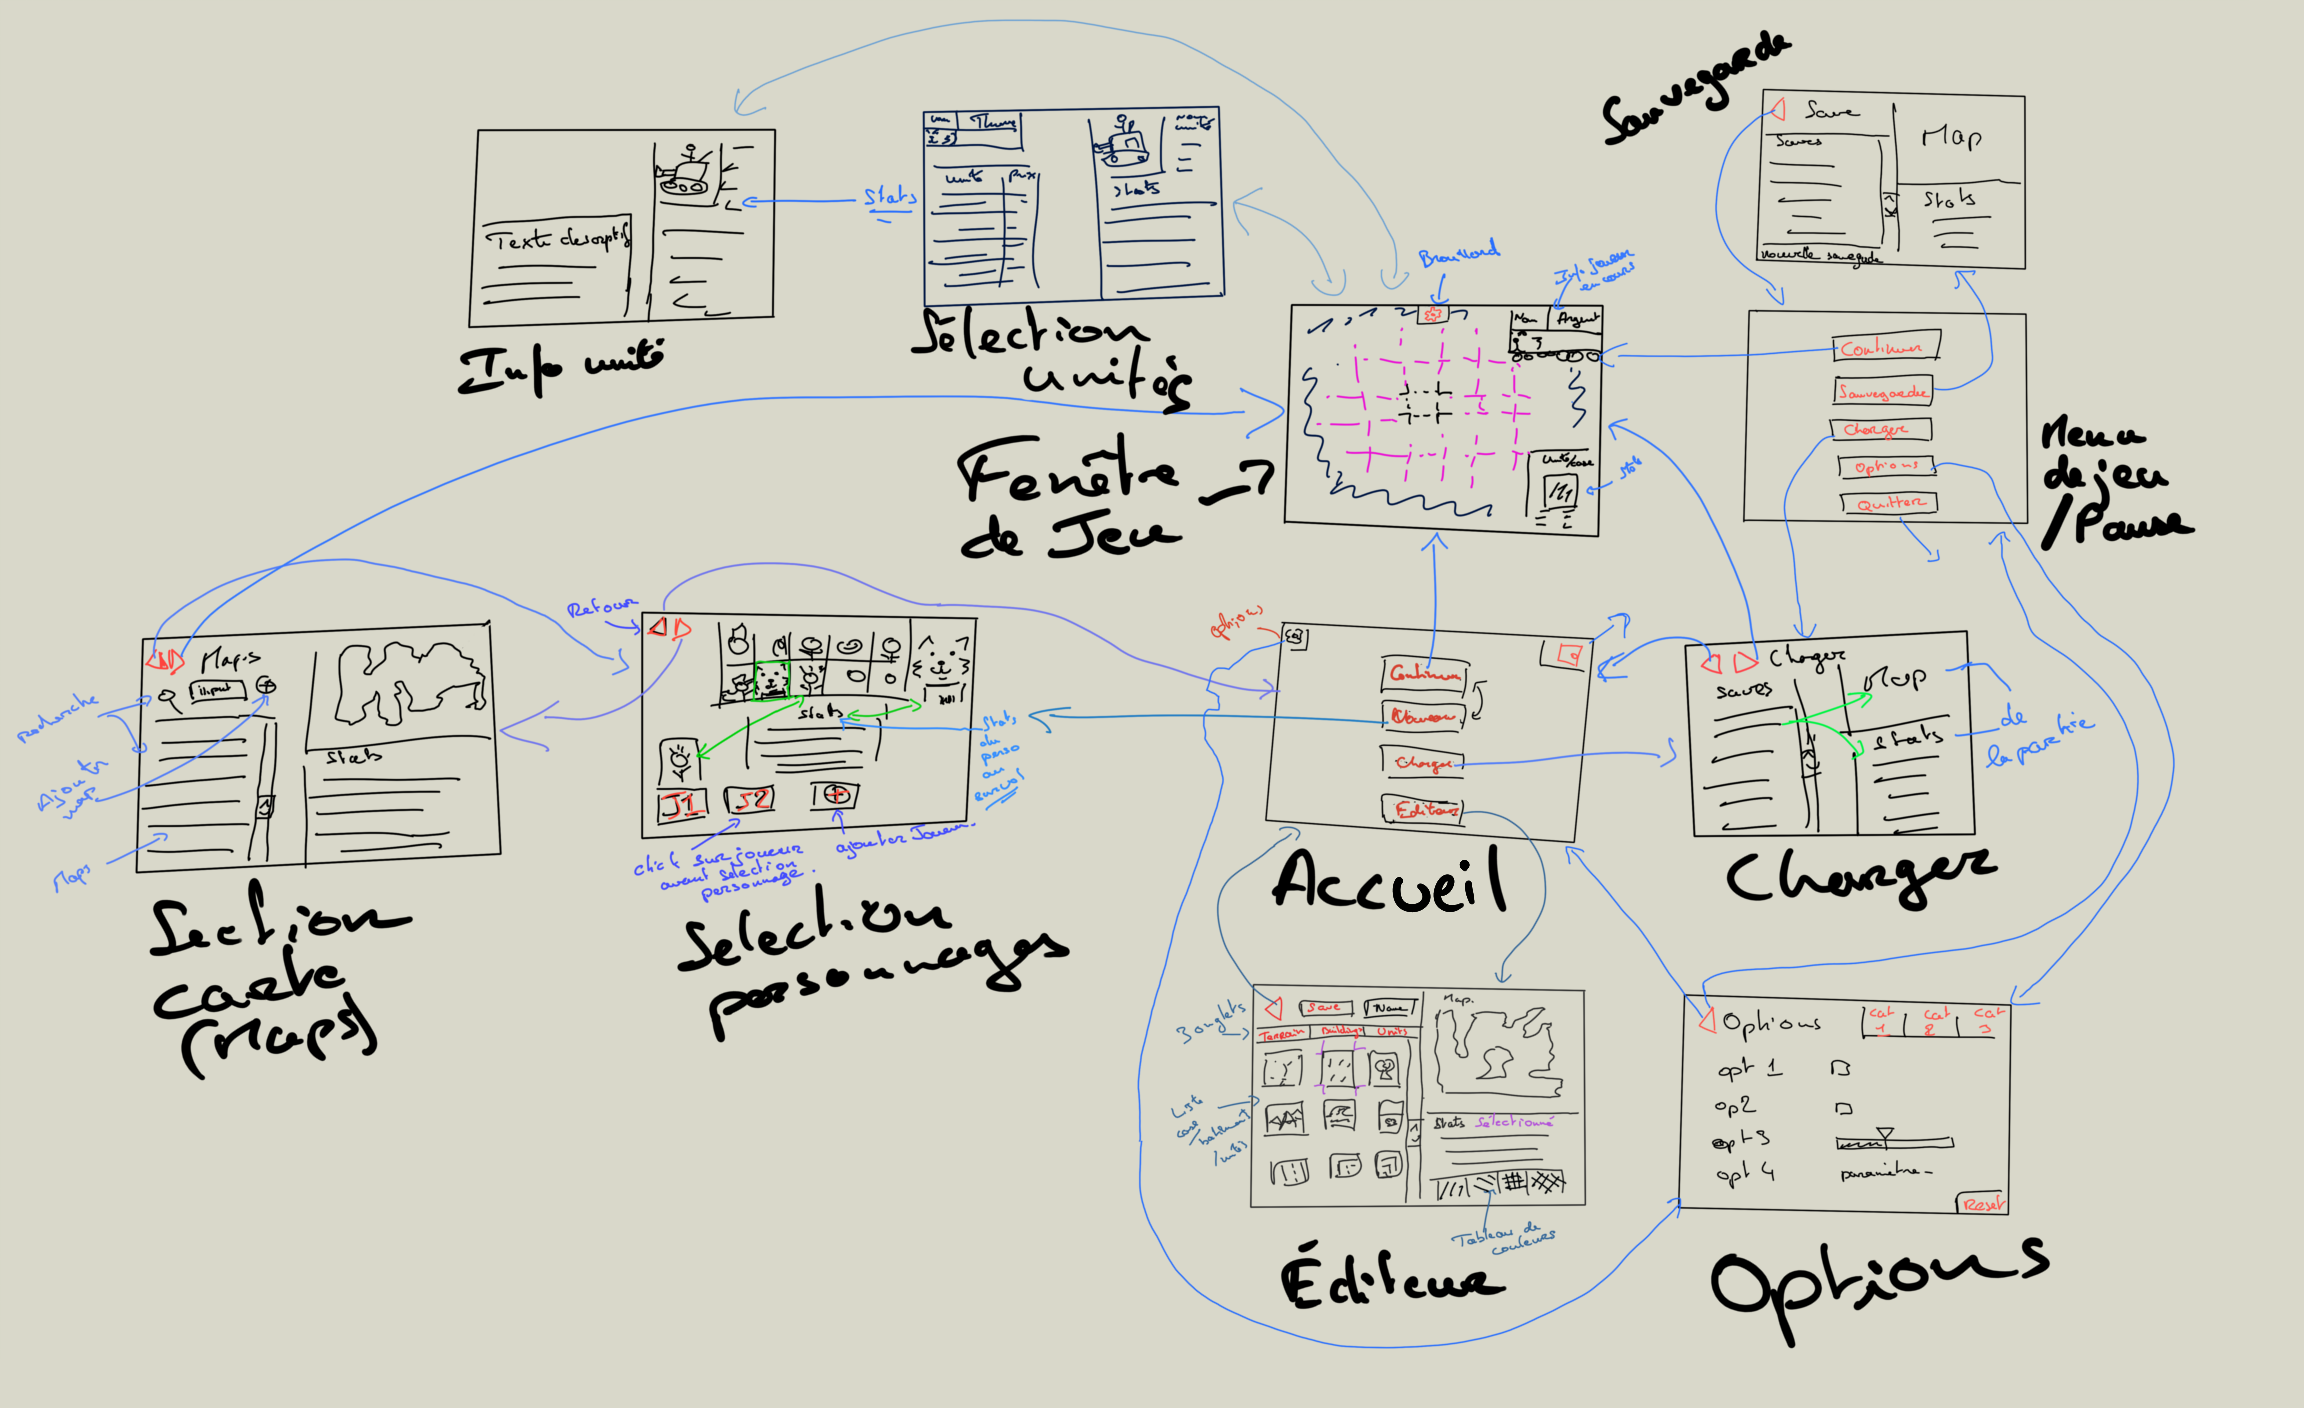
\includegraphics[width=\textwidth]{wireframe}
\subsection{Détail des différentes pages}
\subsubsection{Le menu}
À partir du menu principal nous pouvons (a) continuer la dernière partie jouée, soit (b) en créer une nouvelle, soit (c) charger partie ou enfin (d) aller à l'éditeur de carte.

\begin{enumerate}[label=(\alph*)]
\item nous amène à la fenêtre de jeu dans l'état dans lequel on l'avait laissé
\item à la fenêtre de sélection de personnages pour un nouvelles partie
\item à la liste des parties sauvegardées et qu'on peut reprendre
\item l'éditeur de carte permettra aux utilisateur d'imaginer de nouveaux mondes et de les créer eux même
\end{enumerate}

\subsubsection{Écran de jeu}
En reprenant l'interface du jeu original, nous auront un moteur 2D en fond avec le 'plateau' de jeu, c'est à dire la carte, et au premier plan un curseur qui ciblera toujours une case du plateau et que l'on pourra déplacer au clavier et à la souris. Il y aura aussi deux fenêtre internes plus petites, une dans un coin haut avec l'icône du commandant ou 'personnage' du joueur jouant son tour, et une dans un coin bas qui affichera les détails de la case ciblée par le curseur. La position de ces deux fenêtre variera selon la position du curseur, étant soit dans les coins droit, soit gauche, pour ne pas gêner la visibilité. Par exemple, lorsque le curseur va dans la partie gauche, les fenêtre seront dans la partie droite et vice-versa. Lorsque le curseur se trouve à proximité d'un bord, la carte se déplace dans le sens opposé. On pourra aussi cliquer sur le bouton menu qui sera en haut de l'écran de manière centrée pour accéder au menu général du jeu.

\subsubsection{Création de parties}
La création d'une nouvelle partie se fait en deux étapes soit deux fenêtres. La première est la sélection de son 'personnage' ou commandant. Dans cette première fenêtre nous avons en haut à gauche des boutons en forme de flèche qui nous permettent d'accéder à la fenêtre précédente ou d'accéder à la deuxième étape de la création d'une partie une fois que l'on en a fini avec celle-ci. On nous propose une grille de personnages avec leur statistiques. La première page nous permet d'ajouter des joueurs, de sélectionner les commandant avec lesquels ils souhaitent jouer - en disposant de leur statistiques. Une fois cette étape validé les utilisateur choisissent la carte sur laquelle ils veulent jouer dans une nouvelle fenêtre. Ils peuvent importer des nouvelles cartes et accéder à un rapide descriptif ce ces dernières. 

\subsubsection{Sauvegarde des parties}
Cette page permettra au joueur de sauvegarder sa partie courante dans un fichier. Quand une précédente sauvegarde est sélectionnée pour la réécriture, un aperçut de l'état de la partie déjà sauvegarder s'affiche alors dans la partie droite de la page avec des statistiques de la partie. Ce menu permettra aussi d'effacer une autre partie. Une fois fini, le bouton de retour l'emmènera sur la dernière vue avant qu'il ne soit arrivé dans ce menu.

\subsubsection{Chargement de parties}
Cette page fonctionne de façon analogue à celle des sauvegarde des parties mais permet de charger une partie parmi les sauvegardes.

\subsubsection{Éditeur de niveaux}
Cette page permettra au joueur de créer ses propres cartes ou d'éditer des cartes existantes. il aura un menu tabulé sur la gauche avec toutes les différentes cases possible dans un onglet, les bâtiments dans une deuxième et en fin les unités dans un troisième. Un sélecteur de couleur sera visible en dessous. Dès que le joueur sélectionnera une case du plateau, celle-ci se transformera en la case sectionnée dans le menu. Si c'est une unité qui est alors sélectionnée, cette unité sera placée sur le plateau. Une fois satisfait, le joueur pourra sauvegarder son niveau personnel dans un fichier qui pourra alors être importé lors d'une nouvelle partie. 

Le boutons de retour en haut à gauche permettra de revenir au menu principal.

\subsubsection{Options}
Cette page permettre de configurer manuellement les paramètres du jeu.

\section{Mécaniques de jeu}
\subsection{Les personnages}
Lors d'une partie, chaque joueur choisit un personnage appelé commandant qui va lui fournir des bonus et malus particuliers : il peut améliorer certaines ou toutes les unités, influencer le prix de celles-ci, leur vision, leur portée,... De plus ces commandants ont une jauge de pouvoir qui se charge au fur et à mesure de la partie lorsqu'ils infligent et encaissent des dégâts. Lorsque la jauge est à moitié remplie, le joueur peut utiliser le premier pouvoir du commandant ou alors attendre que celle-ci soit pleine pour utiliser le super-pouvoir qui est plus intéressant que le premier. L'utilisation d'un pouvoir vide la jauge.

\subsection{Les terrains}
Le terrain n'a aucune influence sur les unités aériennes. Tout ce qui est ci-dessous ne s'applique pas à celles-ci. Les unités aériennes peuvent aller sur toutes les cases.\\

Il existe différents types de terrains :

\begin{itemize}
\item Terrestre
\begin{itemize}
\item Forêt (en brouillard de guerre, cache les unités terrestres, défense 2)
\item Montagne (seule l'infanterie peut y aller, augmente le champ de vision, défense 4)
\item Colline (les unités terrestres peuvent y aller, augmente la portée et le champ de vision, défense 2)
\item Plaine (case terrestre 'normale', défense 1)
\item Route (case terrestre sur laquelle le déplacement est facilité, défense 0)
\item Plage (case semi-terrestre permettant l'embarquement des unités dans les barges, défense 0)
\end{itemize}
\item Naval
\begin{itemize}
\item Mer (case maritime 'normale', défense 1)
\item Récif (en brouillard de guerre, cache les unités maritimes, défense 2)
\item Plage (case semi-maritime permettant l'embarquement des unités dans les barges, celles-ci sont les seules unités maritimes à pouvoir y aller, défense 0)
\end{itemize}
\end{itemize}

\subsection{Les unités}
%http://www.aw-experience.com/awds_guides_units.php (détail de la plupart des unités)
On remarque que les unités à distance ne peuvent attaquer et se déplacer dans le même tour. 
On distingue 3 catégories d'unités

\begin{itemize}
\item Les terrestres
\begin{itemize}
    \item Ingénieur : unité pacifique pouvant augmenter de 1 la défense d'une case pour 5 tours ou soigner une unité de 10PV moyennant finance
    \item ensemble des unités militaires qui combattent à pied (Mitrailleuses, Bazooka)
    \item Véhicules : ensemble des unités militaires terrestres motorisées
    \begin{itemize}
        \item VTB : véhicule de transport blindé (transporte une unité d'infanterie et ravitaille)
        \item Recon (Véhicule léger de reconnaissance)
        \item Unités à distance (artillerie et lance-missile)
        \item Unités anti-aériennes
        \begin{itemize}
            \item DCA : unités de contact attaquant les unités terrestres et aériennes
            \item Batterie sol-air : unité à distance anti-aérienne extrêmement efficace
        \end{itemize}
        \item Tanks (véhicules lourds)
        \begin{itemize}
            \item Tank
            \item Tank-M
            \item Néotank
            \item Mégatank
        \end{itemize}
    \end{itemize}
\end{itemize}
\item Les navales
\begin{itemize}
    \item Navires (bateaux standards, à la surface)
    \begin{itemize}
        \item Destroyer (anti-sous-marins, anti-aérien), peut transporter un hélicoptère, résistant aux sous-marins
        \item Cuirassé (très grande portée, attaque les unités terrestres)
        \item Navire de transport
        \item Navire logistique (équivalent naval du VTB pouvant transporter deux unités d'infanterie et soigner 10 PV par tour à une unité adjacente (payant))
        \item Porte-avion : (unité à distance anti-aérienne de très grande portée), transporte deux unités aériennes et les approvisionne quand elles se posent
    \end{itemize}
    \item Sous-marin (peut plonger pour se cacher mais consomme alors plus)
\end{itemize}
\item Les aériennes
\begin{itemize}
    \item Les avions
    \begin{itemize}
        \item Bombardier (unité de contact très puissante, attaque tout sauf l'aérien)
        \item Furtif (unité de contact puissante, pouvant tout attaquer, pouvant se cacher mais consomme alors énormément plus d'essence)
        \item Chasseur (unité anti-aérienne)
    \end{itemize}
    \item Les hélicoptères
    \begin{itemize}
        \item Hélicoptère de combat (attaque tout sauf les avions)
        \item Hélicoptère de transport
        \item Missile balistique (missile se déplaçant sur la carte, de rayon 3 cases, inflige 50 dégâts, explose si n'est pas utilisé avant d'être à court d'essence)
    \end{itemize}
\end{itemize}
\end{itemize}

\subsection{Le déplacement}
Le déplacement de chaque unité dépend du terrain, de son type de mouvement (par exemple les unités terrestres peuvent se déplacer à pied, avec des roues ou des chenilles), du temps (le déplacement est réduit en cas de neige par exemple), des capacités et des commandants (certains commandants peuvent augmenter le déplacement des unités par exemple).

\subsection{Brouillard de guerre et champ de vision}
Le brouillard de guerre peut ou pas être activé sur une carte. Il fait que seules les unités dans le champ de vision des unités et bâtiments du joueur sont vues.\\

Chaque unité a un certain champ de vision qui lui permet de voir autour de sa position, certains terrains comme la forêt ou les récifs permettent aux unités de se cacher (à moins qu'une unité adverse soit adjacente à la case), certains terrains peuvent augmenter la vision des unités comme les montagnes ou les collines. Les unités à distance peuvent tirer à une position qu'elles ne voient pas (contrairement au jeu original).

\subsection{Les bâtiments}
Dans ce jeu les bâtiments sont définis par la carte, impossible d'en construire.

Sauf précisé autrement chaque bâtiment rapport 1000 points par tour. Les bâtiments de production utilisent les points pour produire des unités.

Sauf précisé autrement, chaque bâtiment a une "vie" de 200 points : pour capturer un bâtiment on place une unité d'infanterie dessus et on retire chaque tour la vie de l'unité à la vie du bâtiment, lorsque celle-ci tombe à 0, le bâtiment est capturé par le joueur possédant l'unité d'infanterie. Si un tour se passe sans qu'une unité du même joueur soit sur le bâtiment, celui-ci retrouve sa vie complète (cela permet par exemple de changer l'unité qui prend le bâtiment et de ne pas être bloqué à devoir utiliser la même unité du début à la fin comme dans le jeu original).

\begin{itemize}
\item QG : bâtiment principal du joueur, celui-ci perd si son QG est pris, défense 4
\item Caserne : bâtiment de production d'unités terrestres, défense 3
\item Port : bâtiment de production d'unités maritimes, défense 3
\item Aéroport : bâtiment de production d'unités aériennes, défense 3
\item Ville : bâtiment sans effet particulier, défense 3
\item Silo de missile : case contenant un seul missile pouvant être lancé sur la totalité de la carte, dont le rayon est de 3 cases, défense 2
\end{itemize}

\subsection{Le système de combat}
La vie d'une unité représente la proportion de cette dernière  encore en vie. Les dégâts qu'inflige une unité est donc proportionnelle à sa vie. De plus, les combats fonctionnent avec un système d'armes. C'est à dire que les unités on des armes bien précise qui ne peuvent être utilisées que contre un certain type d'unités ennemies. On remarque que certaines unités de transport, comme le VTB, ne disposent pas d'armes et ne peuvent par conséquent pas attaquer. De la même manière les véhicules d'artillerie ne peuvent pas cibler les unités aériennes.
On note que, bien que les armes aient le même nom, les différentes unités n'infligent pas le mêmes dégâts pour autant. Par exemple, un bazooka fait des dégâts corrects contre les véhicules mais assez faibles contre l’infanterie.
Quand un combat est déclenché l'unité qui attaque profite de l'initiative. C'est à dire qu'elle attaque en premier, la vie du défenseur baisse avant qu'il puisse riposter et, par conséquent elle fait perdre moins de point de vie à l’assaillant. 

$$Damage\%=\left(\frac{B\cdot A_{CO}}{100}+R\right)\cdot\frac{A_{HP}}{10}\cdot \left(\frac{200-D_{CO}-D_{TR}\cdot D_{HP}}{100}\right)$$
$Damage\%$ = Dégâts de base\\
$B$ = Dégâts de base infligé par l'arme\\ 
$A_{CO}$ = Points d'attaque du commandant\\
$R$ = Un nombre aléatoire entre 0 et 9\\
$A_{HP}$ = Nombre de points de vie de l'attaquant\\
$D_{CO}$ = Point de défense du commandant\\
$D_{TR}$ = Point de défense accordé par le terrain\\
$D_{HP}$ = Nombre de points de vie du défenseur\\

Les variables $A_{CO}$ et $D_{CO}$ sont de variables qui dépendent du commandant avec lequel le joueur a décidé de jouer mais aussi de l'unité. Un commandant n'accorde pas le même bonus à tous les types d'unités. Le nombre de points de défense accordé par le terrain est une variable dépendant de l'emplacement sur lequel se trouve l'unité qui défend. Elle compense ainsi l'avantage de l'assaillant qui a l'initiative et rend stratégique des emplacement de la carte.\\


Les unités ne peuvent attaquer en dehors d'une certaines portées. Dans le jeu d'origine on ne peut pas attaquer dans le brouillard de guerre mais nous pensons que c'est assez dommage de ne pas pouvoir viser à l'aveugle. Premièrement, cette règle serait assez peu fidèle avec la réalité. On peut à cet effet évoquer les guerres mondiales ou la guerre du Vietnam. En effet, les bombardements en avion se faisaient souvent à l'aveugle - particulièrement en ce qui concerne la guerre du Vietnam ou la jungle cachais les objectifs. Il est vrai que cet argument "historique" pèse peu dans un jeu de stratégie à l'univers évoquant la science fiction. Cependant, le rapport risque-récompense peut rendre la mécanique intéressante car si on tire dans le vide on perd des munitions notamment pour les véhicules à très longue porté. C'est au moins une piste à explorer.


Les unités disposent pour chaque arme d'un nombre défini de munitions. Ce nombre peut être illimité comme pour l'infanterie ou fini comme pour les tanks. Il faut alors recharger l'unité en munitions. En utilisant soit le VTB, soit aller sur les bâtiments correspondant à l'unité - les casernes, villes et QG pour les unités terrestres, les ports pour les unités navales et aéroport pour les unités aériennes.


\subsection{Évènement aléatoires}
Des évènements aléatoires peuvent se déclencher à un endroit de la carte (et éventuellement se déplacer) :\\

\begin{itemize}
\item Godzilla qui détruit les bâtiments qui ne sont pas des bâtiments de production ou des QG
\item Tornade/typhon qui déplace les unités et/ou inflige des dégâts aux unités maritimes et aériennes
\item Tremblement de terre qui inflige des dégâts aux unités terrestres
\item Faille qui détruit des cases pour quelques tours (on ne peut plus y accéder, les éventuels bâtiments ne peuvent plus produire
\item Révolte (effets à définir plus précisément, principalement l'infanterie est touchée et les unités blessées)
\item Météorite (qui aurait à peu près le même effet qu'un missile)
\end{itemize}

\subsection{Les ressources}
Les ressources du jeu sont au nombre de trois: l'essence, les munitions et l'argent. On récolte ces ressources grâce aux bâtiments. Chaque début de tour, les bâtiments qu'un joueur contrôle lui donne accès à un certain revenu en argent. Les unités ont besoin d'être régulièrement rechargées en essence, sans quoi elle les ne peuvent plus se déplacer. De la même manière sans munitions une unité ne peux plus attaquer ou riposter. On distingue donc deux catégories de ressources: d'une part celles qui sont directement liées à une unité comme l'essence et les munitions et d'un autre côté l'argent qui est globale et lié au joueur. Les dépenses des deux premières ressources se font presque indépendamment de la volonté de joueur alors que ce dernier peut choisir de dépenser sont argent comme il le souhaite. Chaque unité à un coût s'entretient, en essence, et un coût de production. Les unités sont produites dans les bâtiments correspondant à un prix fixé - caserne pour les unités terrestres, port pour les unités navales et aéroport pour les unités 


\end{document}